\chapter{Kompleksasi}\label{ch:b1:complexation}

Tuangkan sedikit larutan amonia ke dalam tembaga(II) sulfat yang biru
pucat: seketika terbentuk endapan biru pucat. Tuangkan lebih banyak lagi,
dan endapan itu larut menjadi larutan berwarna biru pekat, hampir seperti
tinta. Tidak ada satu pun dalam bab asam--basa atau pengendapan yang
menjelaskan tahap kedua itu. Molekul-molekul amonia telah terikat pada
ion tembaga melalui \omterm{def:b1:lewis-resonance-vsepr:lewis}{pasangan elektron bebasnya} dan membentuk spesies
baru, sebuah \omterm{def:b1:complexation:complex}{kompleks}, yang lebih stabil daripada hidroksidanya dan
berwarna lain. \omterm{def:b1:complexation:complex}{Kompleks} mengangkut oksigen di dalam darah, mengikat logam
di dalam klorofil dan vitamin B$_{12}$, melunakkan air sadah, dan
melarutkan logam-logam yang tidak dapat dilarutkan oleh apa pun yang
lain. Bab ini memperlakukannya sebagai satu lagi pertukaran partikel di
dalam air, dengan tetapan dan diagramnya sendiri.

\begin{recall}
\omterm{def:b1:lewis-resonance-vsepr:lewis-acid}{Asam Lewis} (akseptor pasangan elektron), \omterm{def:b1:lewis-resonance-vsepr:lewis-acid}{basa Lewis} (donor pasangan
elektron), dan \omterm{def:b1:lewis-resonance-vsepr:lewis-acid}{ikatan datif} didefinisikan pada
\cref{ch:b1:lewis-resonance-vsepr}. \omterm{def:b1:predominant-reaction:predominance}{Diagram predominansi} dan metode
\omterm{def:b1:predominant-reaction:predominant-reaction}{reaksi predominan} berasal dari \cref{ch:b1:predominant-reaction}; \omterm{def:b1:precipitation:solubility-product}{hasil
kali kelarutan} dan syarat pengendapan dari \cref{ch:b1:precipitation}.
\end{recall}

\begin{omfigure}
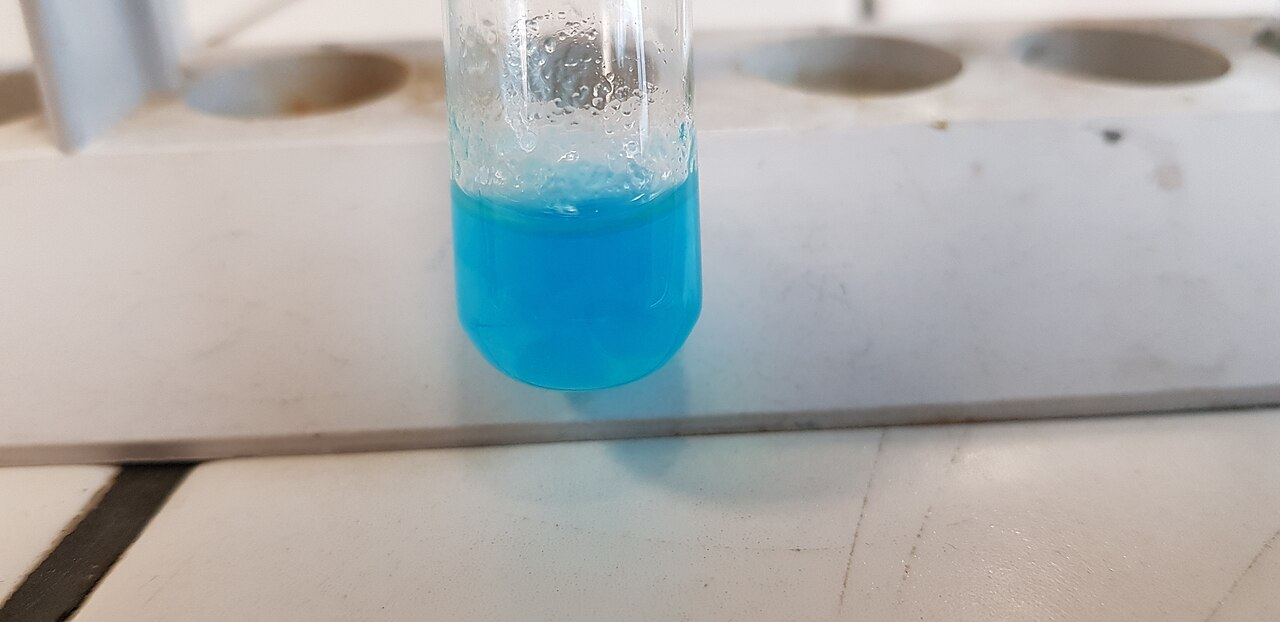
\includegraphics[height=4.2cm]{images/book2/copper-hydroxide.jpg}\hspace{0.6em}%
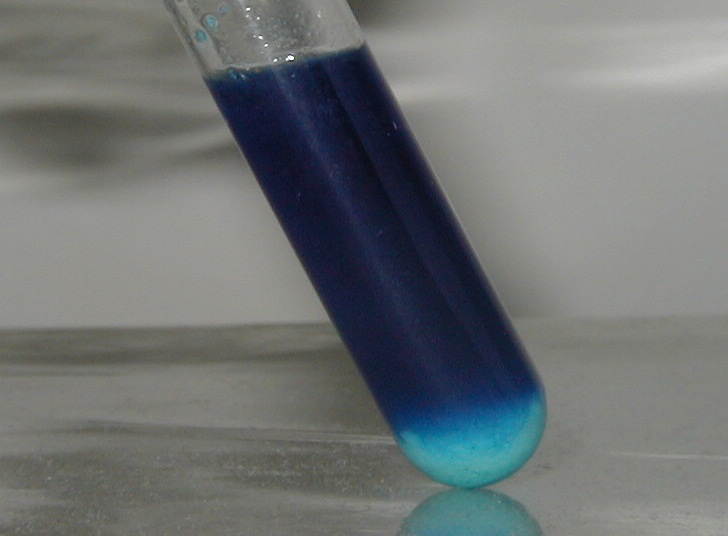
\includegraphics[height=4.2cm]{images/book2/copper-ammine.jpg}

{\small Kiri: suspensi tembaga(II) hidroksida yang biru pucat (foto
Alvy16, CC BY 4.0). Kanan: dengan lebih banyak amonia padatan itu larut
menjadi ion tetraamintembaga(II) yang biru pekat; sebagian hidroksida
yang tidak larut masih berada di dasar tabung (foto Chemicalinterest,
domain publik). Keduanya dari Wikimedia Commons.}
\end{omfigure}

\section{Kompleks dan ligan}

\begin{definition}[Kompleks, atom pusat, ligan]\label{def:b1:complexation:complex}
\emph{Kompleks}\index{kompleks} adalah spesies yang tersusun atas sebuah
\emph{atom pusat}\index{atom pusat} atau ion pusat, biasanya kation logam
yang berperan sebagai \omterm{def:b1:lewis-resonance-vsepr:lewis-acid}{asam Lewis}, yang terikat melalui \omterm{def:b1:lewis-resonance-vsepr:lewis-acid}{ikatan datif} pada
molekul atau ion yang berperan sebagai \omterm{def:b1:lewis-resonance-vsepr:lewis-acid}{basa Lewis}, yaitu
\emph{ligan}\index{ligan}. Rumusnya ditulis di dalam kurung siku, beserta
muatan totalnya: $[\ce{Cu(NH3)4}]^{2+}$,
$[\ce{Fe(CN)6}]^{4-}$, $[\ce{Ag(NH3)2}]^{+}$, $[\ce{FeSCN}]^{2+}$.
\end{definition}

Muatan \omterm{def:b1:complexation:complex}{kompleks} adalah jumlah muatan ion pusat dan muatan \omterm{def:b1:complexation:complex}{ligan-ligannya}:
$\mathrm{Fe^{2+}}$ dan enam \ce{CN-} membentuk
$[\ce{Fe(CN)6}]^{4-}$. Sebuah \omterm{def:b1:complexation:complex}{ligan} memerlukan sedikitnya satu \omterm{def:b1:lewis-resonance-vsepr:lewis}{pasangan
elektron bebas}: \ce{NH3}, \ce{H2O}, \ce{OH-}, \ce{Cl-}, \ce{CN-},
\ce{SCN-} (terikat melalui S atau N). Setiap ion logam di dalam air
sebenarnya sudah merupakan \omterm{def:b1:complexation:complex}{kompleks} dengan molekul-molekul air sebagai
\omterm{def:b1:complexation:complex}{ligan}, $[\ce{Cu(H2O)6}]^{2+}$ atau $[\ce{Fe(H2O)6}]^{3+}$; membentuk
\omterm{def:b1:complexation:complex}{kompleks} lain berarti menukar molekul-molekul air itu dengan \omterm{def:b1:complexation:complex}{ligan} lain,
dan \omterm{def:b1:complexation:complex}{ligan} air tidak dituliskan dalam rumus, sebagaimana \ce{H3O+} ditulis
untuk proton yang terhidrasi.

\begin{omfigure}
\begin{tikzpicture}[font=\small, line cap=round]
  % [Ag(NH3)2]+ : linear
  \begin{scope}
    \node (ag) at (0,0) {\ce{Ag}};
    \node (n1) at (-1.2,0) {\ce{H3N}};
    \node (n2) at (1.2,0) {\ce{NH3}};
    \draw[thick] (n1) -- (ag) -- (n2);
    \node[align=center] at (0,-1.9) {$[\ce{Ag(NH3)2}]^{+}$,\\linear};
  \end{scope}
  % [Cu(NH3)4]2+ : square plane in perspective
  \begin{scope}[xshift=4.3cm, every node/.style={fill=white, inner sep=1.5pt}]
    \node (cu) at (0,0) {\ce{Cu}};
    \node (a) at (-1.45,-0.5) {\ce{H3N}};
    \node (b) at (1.45,0.5) {\ce{NH3}};
    \node (c) at (0.85,-0.9) {\ce{NH3}};
    \node (d) at (-0.85,0.9) {\ce{H3N}};
    \begin{pgfonlayer}{background}
    \draw[gray, dashed] (a.center) -- (c.center) -- (b.center) -- (d.center) -- cycle;
    \end{pgfonlayer}
    \draw[thick] (cu) -- (a); \draw[thick] (cu) -- (b);
    \draw[thick] (cu) -- (c); \draw[thick] (cu) -- (d);
    \node[align=center] at (0,-1.9) {$[\ce{Cu(NH3)4}]^{2+}$,\\segi empat datar};
  \end{scope}
  % [Fe(CN)6]4- : octahedron
  \begin{scope}[xshift=9.2cm, every node/.style={fill=white, inner sep=1.5pt}]
    \node (fe) at (0,0) {\ce{Fe}};
    \node (t) at (0,1.3) {\ce{CN}};
    \node (u) at (0,-1.3) {\ce{CN}};
    \node (l) at (-1.45,-0.45) {\ce{NC}};
    \node (r) at (1.45,0.45) {\ce{CN}};
    \node (f) at (0.8,-0.8) {\ce{CN}};
    \node (k) at (-0.8,0.8) {\ce{NC}};
    \begin{pgfonlayer}{background}
    \draw[gray, dashed] (l.center) -- (f.center) -- (r.center) -- (k.center) -- cycle;
    \end{pgfonlayer}
    \foreach \x in {t,u,l,r,f,k} \draw[thick] (fe) -- (\x);
    \node[align=center] at (0,-1.9) {$[\ce{Fe(CN)6}]^{4-}$,\\oktahedral};
  \end{scope}
\end{tikzpicture}

{\small Tiga \omterm{def:b1:complexation:complex}{kompleks} dan bentuknya. Setiap garis adalah \omterm{def:b1:lewis-resonance-vsepr:lewis-acid}{ikatan datif} dari
\omterm{def:b1:lewis-resonance-vsepr:lewis}{pasangan elektron bebas} \omterm{def:b1:complexation:complex}{ligan} (N pada amonia, C pada sianida) ke ion
logam; garis putus-putus menggambarkan bujur sangkar empat \omterm{def:b1:complexation:complex}{ligan}.
Bentuk-bentuk \omterm{def:b1:complexation:complex}{kompleks} dijelaskan dalam jilid Tahun~2.}
\end{omfigure}

\begin{definition}[Ligan polidentat, kelat]\label{def:b1:complexation:chelate}
\omterm{def:b1:complexation:complex}{Ligan} yang mengikat ion pusat yang sama melalui beberapa atomnya
sekaligus adalah \emph{ligan polidentat}\index{ligan polidentat};
\omterm{def:b1:complexation:complex}{kompleks} yang dibentuknya, yang \omterm{def:b1:complexation:complex}{ligannya} menutup cincin-cincin di sekitar
ion logam, adalah \emph{kelat}\index{kelat}. Etilenadiamina
\ce{H2N-CH2-CH2-NH2} terikat melalui dua atom N, ion oksalat
\ce{C2O4^2-} melalui dua atom O, dan ion etilenadiaminatetraasetat
(\emph{edta}, ditulis \ce{Y^4-}) melalui dua atom N dan empat atom O.
\end{definition}

\begin{omfigure}
\setchemfig{atom sep=1.9em}
\chemfig{N(-[3]-[2]C(=[1]O)-[3]O^{-})(-[5]-[6]C(=[7]O)-[5]O^{-})-[0]-[0]N(-[1]-[2]C(=[3]O)-[1]O^{-})(-[7]-[6]C(=[5]O)-[7]O^{-})}
\hspace{2.2em}
\begin{tikzpicture}[font=\small, baseline=(ca.base)]
  \node[circle, draw, thick, fill=omDef!12, inner sep=1.5pt] (ca) at (0,0) {\ce{Ca}};
  \node (n1) at (-1.15,-0.35) {N};
  \node (n2) at (0.55,-0.6) {N};
  \node (o1) at (0,1.35) {O};
  \node (o2) at (0,-1.35) {O};
  \node (o3) at (1.15,0.35) {O};
  \node (o4) at (-0.55,0.6) {O};
  \foreach \x in {n1,n2,o1,o2,o3,o4} \draw[thick, omDef] (ca) -- (\x);
  \draw[omProp, thick] (n1) .. controls (-0.57,-0.95) .. (n2);
  \draw[omProp, thick] (n1) .. controls (-1.05,0.95) .. (o1);
  \draw[omProp, thick] (n1) .. controls (-1.5,0.25) .. (o4);
  \draw[omProp, thick] (n2) .. controls (0.5,-1.6) .. (o2);
  \draw[omProp, thick] (n2) .. controls (1.5,-0.3) .. (o3);
\end{tikzpicture}

{\small Kiri: ion edta \ce{Y^4-}, dengan kedua atom N dan keempat gugus
karboksilatnya. Kanan: \omterm{def:b1:complexation:chelate}{kelat} kalsium--edta $[\ce{CaY}]^{2-}$, secara
skematis: keenam atom donor (ikatan biru) berada di sudut-sudut sebuah
oktahedron di sekitar ion itu, dengan kedua atom N bersebelahan, dan
rantai-rantai karbon \omterm{def:b1:complexation:complex}{ligan} (jingga) menutup lima cincin yang
masing-masing beranggota lima atom, yaitu cincin-cincin \omterm{def:b1:complexation:chelate}{kelat}.}
\end{omfigure}

Ion edta mengikat ion kalsium cukup kuat untuk menjadi pereaksi titrasi
kesadahan air (\cref{ch:b1:titration-methods}).

\section{Tetapan pembentukan dan tetapan disosiasi}

\begin{definition}[Tetapan pembentukan dan tetapan disosiasi]\label{def:b1:complexation:formation-constant}
Untuk ion pusat M dan \omterm{def:b1:complexation:complex}{ligan} L (muatan tidak dituliskan), \emph{tetapan
pembentukan keseluruhan}\index{tetapan pembentukan keseluruhan}
$\mathrm{ML}_n$ adalah tetapan $\beta_n$ reaksi
$\mathrm{M} + n\,\mathrm{L} \rightleftharpoons \mathrm{ML}_n$,
\[
  \beta_n = \frac{[\mathrm{ML}_n]}{[\mathrm{M}][\mathrm{L}]^n} .
\]
\emph{Tetapan pembentukan bertahap}\index{tetapan pembentukan bertahap}
$K_i$ adalah tetapan penambahan satu \omterm{def:b1:complexation:complex}{ligan},
$\mathrm{ML}_{i-1} + \mathrm{L} \rightleftharpoons \mathrm{ML}_i$.
\emph{Tetapan disosiasi}\index{tetapan disosiasi} adalah kebalikannya,
$K_d = 1/K_i$, dan $\mathrm{p}K_d = \log K_i$, sehingga pasangan
\omterm{def:b1:complexation:complex}{kompleks}/\omterm{def:b1:complexation:complex}{ligan} dipaparkan tepat seperti \omterm{def:b1:predominant-reaction:bronsted}{pasangan asam--basa}, dengan
\omterm{def:b1:complexation:complex}{ligan} menggantikan proton.
\end{definition}

\begin{proposition}[Tetapan keseluruhan dan tetapan bertahap]\label{prop:b1:complexation:beta-k}
$\beta_n = K_1 K_2 \cdots K_n$, yaitu
$\log\beta_n = \sum_{i=1}^n \log K_i$ dan $\log K_i = \log\beta_i -
\log\beta_{i-1}$ (dengan $\beta_0 = 1$).
\end{proposition}

\begin{proof}
Pembentukan $\mathrm{ML}_n$ dari M adalah jumlah $n$ penambahan bertahap;
tetapan jumlah reaksi-reaksi adalah hasil kali tetapan-tetapannya
(\cref{ch:b1:extent-q-and-k}). Hal itu juga terlihat langsung:
$K_1 K_2\cdots K_n = \frac{[\mathrm{ML}]}{[\mathrm{M}][\mathrm{L}]}
\frac{[\mathrm{ML_2}]}{[\mathrm{ML}][\mathrm{L}]}\cdots
\frac{[\mathrm{ML}_n]}{[\mathrm{ML}_{n-1}][\mathrm{L}]}$, dan
konsentrasi zat-zat antaranya saling meniadakan.
\end{proof}

\begin{omfigure}
\begin{tabular}{lll}
\hline
\omterm{def:b1:complexation:complex}{kompleks} & $\log\beta_n$ & $\log K_i$ \\
\hline
$[\ce{Cu(NH3)_n}]^{2+}$, $n = 1$ sampai 4 & 4.10, 7.51, 10.33, 12.36 & 4.10, 3.41, 2.82, 2.03 \\
$[\ce{Ag(NH3)_n}]^{+}$, $n = 1, 2$ & 3.32, 7.22 & 3.32, 3.90 \\
$[\ce{Zn(OH)4}]^{2-}$ & $\log\beta_4 = 14.45$ & \\
$[\ce{FeSCN}]^{2+}$, $[\ce{FeF}]^{2+}$ & 2.96; 6.85 & \\
$[\ce{CaY}]^{2-}$, $[\ce{MgY}]^{2-}$, $[\ce{NiY}]^{2-}$ & 12.69, 10.90, 20.54 & \\
\hline
\end{tabular}

\smallskip
{\small Tetapan pembentukan pada \qty{25}{\celsius}. Tetapan amin, hidrokso,
tiosianato, dan fluoro dihitung dari energi Gibbs pembentukan standar
dalam tabel; tetapan edta adalah nilai-nilai pilihan kritis pada kekuatan
ion nol, demikian pula $\mathrm{p}K_a$ edta yang dipakai di bawah, 2.23,
3.15, 6.80, dan 11.24.}
% ledger: dfg:Cu2+_ao, dfg:CuNH32+_ao, dfg:Cu_NH322+_ao, dfg:Cu_NH332+_ao, dfg:Cu_NH342+_ao, dfg:NH3_ao (computed in figdata/bachelor-1/aqueous-constants.py)
% ledger: dfg:Ag+_ao, dfg:AgNH3+_ao, dfg:Ag_NH32+_ao, dfg:Fe3+_ao, dfg:SCN-_ao, dfg:FeSCN2+_ao, dfg:F-_ao, dfg:FeF2+_ao (computed, same script)
% ledger: logb:Ca-edta, logb:Mg-edta, logb:Ni-edta, pka:edta1, pka:edta2, pka:edta3, pka:edta4
\end{omfigure}

Tetapan bertahap \omterm{def:b1:complexation:complex}{kompleks} amin tembaga mengecil, $K_1 > K_2 > K_3
> K_4$: setiap molekul amonia yang ditambahkan menyisakan lebih sedikit
tempat dan membuat \omterm{def:b1:complexation:complex}{kompleks} itu sedikit kurang bersemangat menerima
molekul berikutnya. Inilah urutan yang biasa. Perak merupakan
pengecualian: $K_2 > K_1$, dengan akibat-akibat yang dibahas dalam soal
akhir pekan.

\section{Predominansi dalam pL}

\begin{definition}[Skala pL]\label{def:b1:complexation:pl-diagram}
Untuk \omterm{def:b1:complexation:complex}{ligan} L, $\mathrm{pL} = -\log[\mathrm{L}]$, dengan $[\mathrm{L}]$
konsentrasi \omterm{def:b1:complexation:complex}{ligan} bebas. \emph{Skala pL}\index{skala pL} adalah sumbu pL
yang padanya digambar daerah-daerah predominansi ion pusat dan
\omterm{def:b1:complexation:complex}{kompleks-kompleksnya}, sebagaimana daerah asam dan basa digambar pada
sumbu pH.
\end{definition}

\begin{proposition}[Batas-batas dalam pL]\label{prop:b1:complexation:pl-boundaries}
Untuk pasangan $\mathrm{ML}_i/\mathrm{ML}_{i-1}$,
\[
  \mathrm{pL} = \log K_i + \log\frac{[\mathrm{ML}_{i-1}]}{[\mathrm{ML}_i]} ,
\]
sehingga $\mathrm{ML}_{i-1}$ predominan untuk $\mathrm{pL} > \log K_i$ dan
$\mathrm{ML}_i$ untuk $\mathrm{pL} < \log K_i$. Jika nilai-nilai
$\log K_i$ mengecil dengan $i$, diagramnya berupa deretan daerah:
$\mathrm{ML}_n$ pada pL kecil (banyak \omterm{def:b1:complexation:complex}{ligan}), lalu $\mathrm{ML}_{n-1}$,
sampai M pada pL besar.
\end{proposition}

\begin{proof}
Ambillah logaritma $K_i = [\mathrm{ML}_i]/([\mathrm{ML}_{i-1}][\mathrm{L}])$:
$\log K_i = \log\frac{[\mathrm{ML}_i]}{[\mathrm{ML}_{i-1}]} + \mathrm{pL}$.
Kedua bentuk sama pada $\mathrm{pL} = \log K_i$, dan rasionya berubah
dengan faktor sepuluh per satuan pL. Daerah $\mathrm{ML}_i$ terletak
antara $\log K_{i+1}$ dan $\log K_i$, yang hanya ada jika $\log K_{i+1} < \log
K_i$.
\end{proof}

\begin{method}[Menggambar diagram pL]\label{met:b1:complexation:pl-diagram}
\begin{enumerate}
  \item Dari nilai-nilai $\log\beta_n$, hitunglah $\log K_i$ bertahap.
  \item Jika nilai-nilai itu mengecil, tempatkan masing-masing pada
        batasnya di sumbu pL: \omterm{def:b1:complexation:complex}{kompleks} dengan \omterm{def:b1:complexation:complex}{ligan} terbanyak di kiri (pL
        kecil), ion bebas di kanan.
  \item Jika ada $\log K_{i+1} > \log K_i$, \omterm{def:b1:complexation:complex}{kompleks} $\mathrm{ML}_i$ tidak
        mempunyai daerah: \omterm{def:b1:complexation:complex}{kompleks} itu bereaksi dengan dirinya sendiri
        menjadi $\mathrm{ML}_{i-1}$ dan $\mathrm{ML}_{i+1}$. Hapuslah
        \omterm{def:b1:complexation:complex}{kompleks} itu dan gambarlah satu batas antara $\mathrm{ML}_{i-1}$
        dan $\mathrm{ML}_{i+1}$ pada
        $\frac12(\log K_i + \log K_{i+1})$.
\end{enumerate}
\end{method}

\begin{omfigure}
\begin{tikzpicture}
\begin{axis}[
  width=0.78\linewidth, height=5.2cm, xmin=0, xmax=7, ymin=0, ymax=1.05,
  axis x line=bottom, axis y line=left, xlabel={$\mathrm{pNH_3}$},
  ylabel={fraksi tembaga},
  tick label style={font=\small}, label style={font=\small}]
\addplot[omThm, thick] table[x=pL, y=M] {figdata/out/bachelor-1-ammine-distribution-copper.dat};
\addplot[omProp, thick] table[x=pL, y=ML] {figdata/out/bachelor-1-ammine-distribution-copper.dat};
\addplot[omMeth, thick] table[x=pL, y=ML2] {figdata/out/bachelor-1-ammine-distribution-copper.dat};
\addplot[black!60, thick] table[x=pL, y=ML3] {figdata/out/bachelor-1-ammine-distribution-copper.dat};
\addplot[omDef, very thick] table[x=pL, y=ML4] {figdata/out/bachelor-1-ammine-distribution-copper.dat};
\node[omDef, font=\small, anchor=west] at (axis cs:0.15,0.78) {$n = 4$};
\node[black!60, font=\small] at (axis cs:2.42,0.63) {3};
\node[omMeth, font=\small] at (axis cs:3.12,0.55) {2};
\node[omProp, font=\small] at (axis cs:3.76,0.58) {1};
\node[omThm, font=\small, anchor=east] at (axis cs:6.9,0.84) {\ce{Cu^2+}};
\end{axis}
\end{tikzpicture}

\begin{tikzpicture}[font=\small, x=1.25cm]
  \draw[->, thick] (0,0) -- (7.2,0) node[right] {$\mathrm{pNH_3}$};
  \foreach \x/\l in {2.03/2.03, 2.82/2.82, 3.41/3.41, 4.10/4.10}
    \draw (\x,0.12) -- (\x,-0.12) node[below] {\l};
  \node[above] at (1.0,0.08) {$[\ce{Cu(NH3)4}]^{2+}$};
  \node[above, font=\scriptsize] at (2.42,0.08) {3};
  \node[above, font=\scriptsize] at (3.12,0.08) {2};
  \node[above, font=\scriptsize] at (3.76,0.08) {1};
  \node[above] at (5.6,0.08) {\ce{Cu^2+}};
  \begin{scope}[yshift=-1.25cm]
  \draw[->, thick] (0,0) -- (7.2,0) node[right] {$\mathrm{pNH_3}$};
  \draw (3.61,0.12) -- (3.61,-0.12) node[below] {3.61};
  \draw[dotted] (3.32,0.3) -- (3.32,-0.1); \draw[dotted] (3.90,0.3) -- (3.90,-0.1);
  \node[above] at (1.6,0.08) {$[\ce{Ag(NH3)2}]^{+}$};
  \node[above] at (5.4,0.08) {\ce{Ag+}};
  \end{scope}
\end{tikzpicture}

{\small Atas: fraksi tembaga(II) yang berada sebagai \ce{Cu^2+} dan
sebagai $[\ce{Cu(NH3)_n}]^{2+}$ ($n = 1$ sampai 4) terhadap
$\mathrm{pNH_3}$. Tengah: \omterm{def:b1:predominant-reaction:predominance}{diagram predominansi} \omterm{def:b1:complexation:complex}{kompleks} amin tembaga,
dengan batas-batas pada $\log K_i$. Bawah: perak, dengan
$\log K_2 = 3.90 > \log K_1 = 3.32$ (titik-titik): $[\ce{AgNH3}]^{+}$
tidak mempunyai daerah dan satu-satunya batas terletak pada
$\frac12\log\beta_2 = 3.61$.}
\end{omfigure}

\begin{example}[Tembaga dalam amonia \texorpdfstring{\qty{0.010}{mol/L}}{0.010 mol/L}]\label{ex:b1:complexation:cu}
Jika amonia bebas $[\ce{NH3}] = \qty{0.010}{mol/L}$, $\mathrm{pNH_3} = 2.0$
terletak di daerah $[\ce{Cu(NH3)3}]^{2+}$, tetapi dekat dengan batas 2.03
terhadap $[\ce{Cu(NH3)4}]^{2+}$: keduanya hampir sama. Fraksi-fraksinya
sebanding dengan $\beta_n[\ce{NH3}]^n = 10^{\log\beta_n - 2n}$, yaitu
$1 : 10^{2.10} : 10^{3.51} : 10^{4.33} : 10^{4.36}$, sehingga \qty{48}{\percent}
$[\ce{Cu(NH3)4}]^{2+}$, \qty{45}{\percent} $[\ce{Cu(NH3)3}]^{2+}$,
\qty{7}{\percent} $[\ce{Cu(NH3)2}]^{2+}$, dan hampir tidak ada \ce{Cu^2+}
bebas.
\end{example}

\section{Persaingan}

Sebuah \omterm{def:b1:complexation:complex}{ligan} dapat diperebutkan oleh dua ion logam, sebuah ion logam oleh
dua \omterm{def:b1:complexation:complex}{ligan}, dan keduanya juga terlibat dalam kesetimbangan pengendapan dan
asam--basa. Setiap persaingan adalah satu reaksi lagi yang tetapannya
menggabungkan tetapan-tetapan yang sudah diketahui; metode \omterm{def:b1:predominant-reaction:predominant-reaction}{reaksi
predominan} pada \cref{ch:b1:predominant-reaction} lalu berlaku tanpa
perubahan.

\begin{example}[Dua ligan untuk besi(III)]\label{ex:b1:complexation:scn-f}
Setetes tiosianat dalam larutan besi(III) menghasilkan
$[\ce{FeSCN}]^{2+}$ yang merah darah; ion fluorida menghilangkan warnanya:
\[
  [\ce{FeSCN}]^{2+} + \ce{F-} \rightleftharpoons [\ce{FeF}]^{2+} + \ce{SCN-},
  \qquad K = \frac{\beta(\ce{FeF})}{\beta(\ce{FeSCN})} = 10^{6.85 - 2.96} =
  10^{3.89} .
\]
\omterm{def:b1:complexation:complex}{Kompleks} yang lebih kuat ($\beta$ lebih besar) mengambil ion logamnya,
tepat seperti asam yang lebih kuat memberikan protonnya kepada basa yang
lebih kuat.
\end{example}

\begin{proposition}[Kompleksasi melawan pengendapan]\label{prop:b1:complexation:competition-precipitation}
Padatan MX larut dalam \omterm{def:b1:complexation:complex}{ligan} L melalui
$\mathrm{MX(s)} + n\,\mathrm{L} \rightleftharpoons \mathrm{ML}_n + \mathrm{X}$,
dengan tetapan $K = \beta_n K_s$. Jika \omterm{def:b1:complexation:complex}{kompleks} itu satu-satunya bentuk M
dalam larutan dan konsentrasi \omterm{def:b1:complexation:complex}{ligan} bebasnya $[\mathrm{L}]$, \omterm{def:b1:precipitation:solubility}{kelarutannya}
adalah $s = \sqrt{K}\,[\mathrm{L}]^{n/2}$.
\end{proposition}

\begin{proof}
Reaksi itu adalah jumlah pelarutan (tetapan $K_s$) dan pembentukan
$\mathrm{ML}_n$ ($\beta_n$). Pada keadaan jenuh $[\mathrm{ML}_n]
= [\mathrm{X}] = s$ dan $K = s^2/[\mathrm{L}]^n$.
\end{proof}

\begin{method}[Melarutkan endapan melalui kompleksasi]\label{met:b1:complexation:dissolve-precipitate}
\begin{enumerate}
  \item Tuliskan reaksi pelarutan menjadi \omterm{def:b1:complexation:complex}{kompleks} dan hitunglah
        $K = \beta_n K_s$.
  \item Jika $K$ besar, pelarutannya \omterm{def:b1:extent-q-and-k:quantitative}{kuantitatif} selama \omterm{def:b1:complexation:complex}{ligan} cukup
        tersedia; jika kecil, hitunglah konsentrasi \omterm{def:b1:complexation:complex}{ligan} bebas yang
        diperlukan agar jumlah padatan itu larut:
        $[\mathrm{L}]^n = s^2/K$.
  \item Tambahkan \omterm{def:b1:complexation:complex}{ligan} yang terikat dalam \omterm{def:b1:complexation:complex}{kompleks}, $n s$, untuk
        memperoleh jumlah total \omterm{def:b1:complexation:complex}{ligan} yang harus dimasukkan.
  \item Periksalah bahwa ion logam bebas dapat diabaikan:
        $[\mathrm{M}] = K_s/s
        \ll s$.
\end{enumerate}
\end{method}

Dengan amonia, perak klorida ($K = 10^{7.22 - 9.75} = 10^{-2.53}$) larut
dalam larutan yang cukup pekat, sedangkan perak iodida
($K = 10^{-8.85}$) tidak: soal akhir pekan memakai hal ini untuk
membedakan halida-halida itu.

\begin{proposition}[Kompleksasi melawan keasaman]\label{prop:b1:complexation:ligand-acidity}
Jika \omterm{def:b1:complexation:complex}{ligan} itu basa $\mathrm{L}$ dari sebuah asam $\mathrm{HL}$ (dan
mungkin bentuk-bentuk yang lebih terprotonasi), hanya bagian
$[\mathrm{L}]/c_L =
1/\alpha$ dari \omterm{def:b1:complexation:complex}{ligan} yang tidak terikat pada logam
yang tersedia, dengan
\[
  \alpha = 1 + \frac{[\ce{H3O+}]}{K_{an}} + \frac{[\ce{H3O+}]^2}{K_{an}K_{a(n-1)}}
  + \cdots
\]
($K_{an}$ \omterm{def:b1:predominant-reaction:acidity-constant}{tetapan keasaman} terakhir). Pada pH tetap, kompleksasi lalu
berperilaku seakan-akan tetapannya adalah tetapan \emph{kondisional}
$\beta' = \beta/\alpha$, yang makin kecil makin rendah pH-nya.
\end{proposition}

\begin{proof}
\omterm{def:b1:complexation:complex}{Ligan} yang tidak terikat pada logam terbagi di antara L, HL, \ce{H2L}, dan
seterusnya, dengan $[\mathrm{HL}] = [\mathrm{L}][\ce{H3O+}]/K_{an}$ dan
hubungan yang serupa untuk bentuk-bentuk berikutnya
(\cref{ch:b1:predominant-reaction}). Dengan menjumlahkannya diperoleh
$c_L = \alpha[\mathrm{L}]$,
dan $\beta = [\mathrm{ML}]/([\mathrm{M}][\mathrm{L}]) =
\alpha[\mathrm{ML}]/([\mathrm{M}]c_L)$, sehingga $[\mathrm{ML}]/([\mathrm{M}]c_L)
= \beta/\alpha$.
\end{proof}

Untuk edta pada pH 10, $\alpha = 1 + 10^{11.24 - 10} + 10^{11.24 + 6.80 - 20}
= 18.4$, sehingga \omterm{def:b1:complexation:complex}{kompleks} kalsium mempertahankan
$\log\beta' = 12.69 - 1.26 = 11.43$; pada pH 7 nilainya turun menjadi
8.24 (\cref{exo:b1:complexation:9}). Itulah sebabnya titrasi kalsium
dengan edta dijalankan dalam penyangga amonia pada pH 10. Amonia pun
sebuah basa: dalam asam amonia menjadi \ce{NH4+}, yang tidak mempunyai
\omterm{def:b1:lewis-resonance-vsepr:lewis}{pasangan elektron bebas}, dan \omterm{def:b1:complexation:complex}{kompleks-kompleks} amin terurai. Penambahan
asam nitrat ke $[\ce{Ag(NH3)2}]^{+}$ dengan adanya klorida memunculkan
kembali endapan putih perak klorida.

Larutan pengikat (fiksatif) fotografi melakukan hal yang sama dengan
\omterm{def:b1:complexation:complex}{ligan} lain ion perak, yaitu ion tiosulfat \ce{S2O3^2-}: larutan itu
melarutkan perak halida yang tidak terkena cahaya, sehingga gambarnya
tidak lagi menggelap. Tetapan-tetapannya tidak termasuk data jilid ini;
amonia memperlihatkan kimia yang sama dengan perak klorida.

\section{Latihan}

\begin{exercise}[$\star$]\label{exo:b1:complexation:1}
Untuk setiap \omterm{def:b1:complexation:complex}{kompleks} berikut, tentukan ion pusat, muatannya, \omterm{def:b1:complexation:complex}{ligan-ligan},
dan atom yang dipakai setiap \omterm{def:b1:complexation:complex}{ligan} untuk berikatan:
$[\ce{Cu(NH3)4}]^{2+}$,
$[\ce{Fe(CN)6}]^{4-}$, $[\ce{Fe(CN)6}]^{3-}$, $[\ce{Ag(NH3)2}]^{+}$,
$[\ce{FeSCN}]^{2+}$, $[\ce{Zn(OH)4}]^{2-}$, $[\ce{CaY}]^{2-}$.
\end{exercise}

\begin{exercise}[$\star$]\label{exo:b1:complexation:2}
Dari nilai-nilai $\log\beta_n$ \omterm{def:b1:complexation:complex}{kompleks} amin tembaga, hitunglah keempat
$\log K_i$ dan keempat $\mathrm{p}K_d$. Tuliskan reaksi disosiasi yang
dirujuk oleh $\mathrm{p}K_d$ terakhir.
\end{exercise}

\begin{exercise}[$\star$]\label{exo:b1:complexation:3}
Gambarlah diagram pL \omterm{def:b1:complexation:complex}{kompleks} amin tembaga. Spesies tembaga manakah yang
predominan pada $[\ce{NH3}] = 1.0$, \num{3.2e-3}, \num{3.2e-4}, dan
\qty{1.0e-5}{mol/L}?
\end{exercise}

\begin{exercise}[$\star$]\label{exo:b1:complexation:4}
Sebuah larutan mengandung besi(III) \qty{1.0e-3}{mol/L} dan tiosianat
\qty{0.10}{mol/L}. Dengan mengabaikan tiosianat yang terikat, berapa
bagian besi yang berada sebagai $[\ce{FeSCN}]^{2+}$?
\end{exercise}

\begin{exercise}[$\star\star$]\label{exo:b1:complexation:5}
Buktikan bahwa dalam larutan ion logam M dan \omterm{def:b1:complexation:complex}{kompleks-kompleksnya}
$\mathrm{ML}_n$, fraksi $\mathrm{ML}_n$ adalah
$\beta_n[\mathrm{L}]^n / \sum_{k} \beta_k[\mathrm{L}]^k$. Tunjukkan
bahwa, jika hanya $\mathrm{ML}_{i-1}$, $\mathrm{ML}_i$, dan
$\mathrm{ML}_{i+1}$ yang hadir dalam jumlah berarti, fraksi
$\mathrm{ML}_i$ paling besar ketika $[\mathrm{ML}_{i-1}] = [\mathrm{ML}_{i+1}]$,
pada $\mathrm{pL} = \frac12(\log K_i + \log K_{i+1})$, lalu hitunglah pNH3
ini untuk $[\ce{Cu(NH3)2}]^{2+}$.
\end{exercise}

\begin{exercise}[$\star\star$]\label{exo:b1:complexation:6}
Ke dalam larutan merah pada \cref{exo:b1:complexation:4} ditambahkan
natrium fluorida sampai $[\ce{F-}] = \qty{0.010}{mol/L}$ (bebas).
Hitunglah tetapan pertukaran \omterm{def:b1:complexation:complex}{ligannya} dan rasio
$[\ce{FeF^2+}]/[\ce{FeSCN^2+}]$. Apa yang terlihat?
\end{exercise}

\begin{exercise}[$\star\star$]\label{exo:b1:complexation:7}
Ion kalsium ditambahkan ke dalam larutan $[\ce{MgY}]^{2-}$, dalam jumlah
yang sama. Tuliskan reaksi pertukarannya, hitunglah tetapannya, dan
bagian magnesium yang dibebaskan.
\end{exercise}

\begin{exercise}[$\star\star$]\label{exo:b1:complexation:8}
Perak oksida \ce{Ag2O} adalah padatan cokelat: \ce{Ag2O(s) + H2O <=> 2Ag+ + 2OH-}
mempunyai $\mathrm{p}K = 15.43$. Tuliskan pelarutannya dalam amonia
menjadi $[\ce{Ag(NH3)2}]^{+}$, hitunglah tetapannya, lalu jelaskan
mengapa endapan cokelat yang terbentuk oleh sedikit amonia dalam perak
nitrat larut dalam amonia yang lebih banyak.
\end{exercise}

\begin{exercise}[$\star\star$]\label{exo:b1:complexation:9}
Hitunglah $\alpha$ dan tetapan kondisional $\log\beta'$ $[\ce{CaY}]^{2-}$
pada pH 10 dan pada pH 7 (\cref{prop:b1:complexation:ligand-acidity}).
Mengapa titrasi kalsium dengan edta mustahil dalam larutan netral jika
diperlukan tetapan kondisional sedikitnya $10^{10}$?
\end{exercise}

\begin{exercise}[$\star\star\star$]\label{exo:b1:complexation:10}
Tembaga(II) oksida \ce{CuO} adalah padatan yang terbentuk dari tembaga(II)
hidroksida jika didiamkan; \ce{CuO(s) + H2O <=> Cu^2+ + 2OH-} mempunyai
$\mathrm{p}K = 20.64$.
\begin{enumerate}
  \item Tuliskan pelarutan \ce{CuO} dalam amonia menjadi
        $[\ce{Cu(NH3)4}]^{2+}$ dan hitunglah tetapannya.
  \item Dalam amonia \qty{1.0}{mol/L} saja, pH ditentukan oleh amonia
        ($\mathrm{p}K_a(\ce{NH4+}) = 9.25$). Hitunglah pH dan konsentrasi
        tembaga yang larut.
  \item Pertanyaan yang sama dalam penyangga amonia dan amonium klorida,
        keduanya \qty{1.0}{mol/L}. Simpulkan.
\end{enumerate}
\end{exercise}

\begin{exercise}[$\star\star\star$]\label{exo:b1:complexation:11}
Perak dan amonia.
\begin{enumerate}
  \item Tunjukkan bahwa $[\ce{AgNH3}]^{+}$ bereaksi dengan dirinya sendiri,
        \ce{2[AgNH3]+ <=> Ag+ + [Ag(NH3)2]+}, lalu hitunglah tetapannya.
  \item Hitunglah fraksi perak terbesar yang pernah berada sebagai
        $[\ce{AgNH3}]^{+}$, serta pNH3 tempat hal itu terjadi.
\end{enumerate}
\end{exercise}

\begin{exercise}[$\star\star\star$]\label{exo:b1:complexation:12}
Larutan edta, \qty{0.10}{mol/L} \ce{Y^4-} pada pH tinggi, dipakai untuk
melarutkan kerak kalsium karbonat.
\begin{enumerate}
  \item Tuliskan reaksinya dan hitunglah tetapannya.
  \item Berapa massa kalsium karbonat yang dapat dilarutkan satu liter?
  \item Mengapa larutan itu harus basa? (Karbonat dan ion edta
        keduanya basa.)
\end{enumerate}
\end{exercise}

\section{Soal: Amonia dan Ketiga Perak Halida}

\begin{problem}[{Soal akhir pekan --- kompleks amin perak dan tetapannya
yang terbalik, pelarutan perak klorida, bromida, dan iodida dalam amonia,
uji penegasan, dan amonia paling sedikit yang melarutkan satu gram perak
klorida}]
\label{pb:b1:complexation:1}
Seorang analis mempunyai tiga endapan putih sampai kuning dan harus
menentukan mana yang perak klorida, perak bromida, dan perak iodida;
lalu ia harus melarutkan \qty{1.0}{g} perak klorida dalam \qty{1.00}{L}
dengan amonia sesedikit mungkin. Data pada \qty{25}{\celsius}:
$\log\beta_1 = 3.32$ dan $\log\beta_2 = 7.22$ untuk \omterm{def:b1:complexation:complex}{kompleks} amin perak;
$\mathrm{p}K_s$ \ce{AgCl} 9.75, \ce{AgBr} 12.27, \ce{AgI} 16.07;
$\mathrm{p}K_a(\ce{NH4+}) = 9.25$; massa molar \ce{AgCl}
\qty{143.4}{g/mol}, \ce{AgBr} \qty{187.8}{g/mol}, \ce{AgI}
\qty{234.8}{g/mol}.

\medskip
\noindent\textbf{Bagian I --- \omterm{def:b1:complexation:complex}{Kompleks} amin perak.}
\begin{enumerate}
  \item Tuliskan reaksi pembentukan $[\ce{AgNH3}]^{+}$ dan
        $[\ce{Ag(NH3)2}]^{+}$ serta ungkapan $\beta_1$ dan $\beta_2$.
  \item Hitunglah $\log K_1$ dan $\log K_2$.
  \item Gambarlah diagram pL secara naif dengan kedua batas ini. Apa yang
        salah di dalamnya?
  \item Tuliskan reaksi $[\ce{AgNH3}]^{+}$ dengan dirinya sendiri dan
        hitunglah tetapannya.
  \item Gambarlah diagram yang benar; di manakah satu-satunya batasnya?
  \item Pada $[\ce{NH3}] = \qty{0.10}{mol/L}$, hitunglah
        $[\ce{Ag(NH3)2+}]/[\ce{Ag+}]$.
  \item Tentukan \omterm{def:b1:complexation:formation-constant}{tetapan disosiasi} keseluruhan $\mathrm{p}K_d$
        $[\ce{Ag(NH3)2}]^{+}$.
\end{enumerate}

\medskip
\noindent\textbf{Bagian II --- Perak klorida dalam amonia.}
\begin{enumerate}[resume]
  \item Tuliskan pelarutan \ce{AgCl} dalam amonia dan hitunglah
        tetapannya.
  \item Nyatakan \omterm{def:b1:precipitation:solubility}{kelarutan} $s$ sebagai fungsi konsentrasi amonia bebas
        dan hitunglah untuk $[\ce{NH3}] = \qty{1.0}{mol/L}$.
  \item Seberapa besar \omterm{def:b1:precipitation:solubility}{kelarutan} itu bertambah dibandingkan dengan di
        dalam air murni?
  \item Berapa massa perak klorida yang kemudian dilarutkan satu liter?
  \item Periksalah bahwa \ce{Ag+} bebas dapat diabaikan.
  \item Sekarang \qty{1.0}{mol/L} adalah amonia total yang dimasukkan.
        Dengan memperhitungkan amonia yang terikat, hitunglah $s$ lagi.
  \item Amonia adalah basa; jelaskan mengapa protonasinya dapat diabaikan
        dalam larutan ini.
\end{enumerate}

\medskip
\noindent\textbf{Bagian III --- Bromida dan iodida.}
\begin{enumerate}[resume]
  \item Hitunglah tetapan pelarutan \ce{AgBr} dalam amonia.
  \item Hitunglah \omterm{def:b1:precipitation:solubility}{kelarutan} \ce{AgBr} dalam amonia bebas
        \qty{1.0}{mol/L}, dalam \unit{mol/L} dan \unit{g/L}.
  \item Hal yang sama untuk \ce{AgI}, dalam \unit{mg/L}.
  \item Turunkan cara mengenali ketiga endapan itu.
  \item Konsentrasi amonia bebas berapakah yang akan melarutkan
        \qty{1.0}{g} \ce{AgBr} dalam \qty{1.00}{L}?
  \item Hal yang sama untuk \qty{1.0}{g} \ce{AgI}. Berikan komentar.
\end{enumerate}

\medskip
\noindent\textbf{Bagian IV --- Satu gram perak klorida.}
\begin{enumerate}[resume]
  \item Ke dalam larutan amoniakal perak klorida ditambahkan asam nitrat.
        Tuliskan reaksi keseluruhannya dan hitunglah tetapannya. Apa yang
        dilihat analis itu?
  \item Konsentrasi amonia bebas berapakah yang diperlukan untuk
        melarutkan \qty{1.0}{g} \ce{AgCl} dalam \qty{1.00}{L}?
  \item Berapa banyak amonia yang terikat dalam \omterm{def:b1:complexation:complex}{kompleks}?
  \item Periksalah bahwa \ce{Ag+} bebas dapat diabaikan dalam larutan ini.
  \item Berapa konsentrasi total amonia paling kecil yang melarutkan
        \qty{1.0}{g} perak klorida dalam \qty{1.00}{L}?
\end{enumerate}
\end{problem}
